To test if an increase on the deepness of the network would improve its results, four networks using two convolutional layers were experimented. 

At the ``CCL'' network, the first convolutional layer uses 8 units for the input window, and a stride of the same size, thus dividing the 512 bytes of the input block in 64 matrices of 8x256 that are then converted in 64 vectors of 128 units. The second layer divides the 64x128 input in 8 matrices of 8x128, producing 8 vectors of 64 units. The LSTM layer uses each of these 8 vectors as time steps, producing a single vector of 3 units, one for each class.

The ``CCLL'' network adds a LSTM layer of 64 output units between the convolutional layers and the final LSTM layer.

The ``CMCML'' network is similar to ``CCL'', but uses max pooling of size 2 at each convolutional layer. This max pooling act on the second dimension instead of the first, and thus does not change the number of steps that the LSTM layer will process. For example, the first max pooling halves the number of output units of the first convolutional layer from 128 to 64.

The ``CMCMLL'' network combines the two additions, using max pooling and using two LSTM layers.

The results are shown in table \ref{tab:carving2convs}. The ``CL'' network is included for comparison. The  ``CL'' network results were only better than the the ``CCL'' network. The other three networks presented better accuracy values, as can be seen in figure \ref{fig:nolstm}.The ``CMCML'' and ``CMCMLL'' results were similar.

\begin{table}[!ht]
    \centering
    \caption[Two convolutional layers]{Comparison of models that use two convolutional layers}
    \label{tab:carving2convs}
\begin{tabular}{r|r|r|r|r|r|r}
\hline
Name & Parameters & Blocks & Epochs & Time & Training          & Validation          \\       
     &            &        &        &         &          accuracy &            accuracy \\ \hline\hline

CL	    & 24663	    & all	& 150	& 9m29s	    & 0.798	& 0.756 \\\hline
CCL	    & 328688	& all	& 150	& 8m29s	    & 0.782	& 0.804 \\\hline
CCLL	& 361712	& all	& 144	& 10m01s	& 0.868	& 0.833 \\\hline
CMCML	& 295536	& all	& 110	& 6m50s	    & 0.904	& 0.88 \\\hline
CMCMLL	& 320752	& all	& 101	& 7m44s	    & 0.905	& 0.875 \\\hline
\end{tabular}
\end{table}

\begin{figure}[htb!]
\centering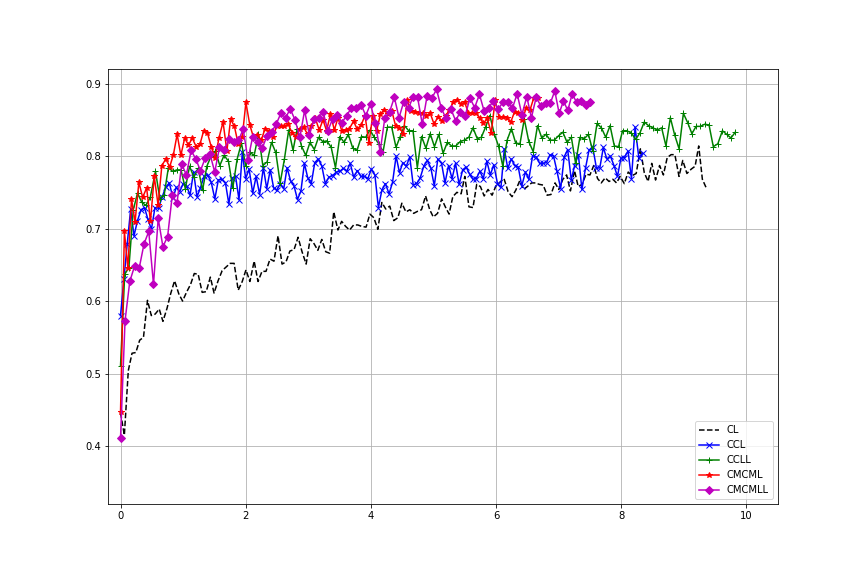
\includegraphics[width=0.65\textwidth]{content/CL-CCL-CCLL-CMCML-CMCMLL.png}
\caption[Two convolutional layers]{\label{fig:twoconvs}Comparison of models that use two convolutional layers - accuracy vs. time(minutes)}
\end{figure}
